% Options for packages loaded elsewhere
\PassOptionsToPackage{unicode}{hyperref}
\PassOptionsToPackage{hyphens}{url}
\PassOptionsToPackage{dvipsnames,svgnames,x11names}{xcolor}
%
\documentclass[
  letterpaper,
  DIV=11,
  numbers=noendperiod]{scrartcl}

\usepackage{amsmath,amssymb}
\usepackage{iftex}
\ifPDFTeX
  \usepackage[T1]{fontenc}
  \usepackage[utf8]{inputenc}
  \usepackage{textcomp} % provide euro and other symbols
\else % if luatex or xetex
  \usepackage{unicode-math}
  \defaultfontfeatures{Scale=MatchLowercase}
  \defaultfontfeatures[\rmfamily]{Ligatures=TeX,Scale=1}
\fi
\usepackage{lmodern}
\ifPDFTeX\else  
    % xetex/luatex font selection
\fi
% Use upquote if available, for straight quotes in verbatim environments
\IfFileExists{upquote.sty}{\usepackage{upquote}}{}
\IfFileExists{microtype.sty}{% use microtype if available
  \usepackage[]{microtype}
  \UseMicrotypeSet[protrusion]{basicmath} % disable protrusion for tt fonts
}{}
\makeatletter
\@ifundefined{KOMAClassName}{% if non-KOMA class
  \IfFileExists{parskip.sty}{%
    \usepackage{parskip}
  }{% else
    \setlength{\parindent}{0pt}
    \setlength{\parskip}{6pt plus 2pt minus 1pt}}
}{% if KOMA class
  \KOMAoptions{parskip=half}}
\makeatother
\usepackage{xcolor}
\setlength{\emergencystretch}{3em} % prevent overfull lines
\setcounter{secnumdepth}{5}
% Make \paragraph and \subparagraph free-standing
\ifx\paragraph\undefined\else
  \let\oldparagraph\paragraph
  \renewcommand{\paragraph}[1]{\oldparagraph{#1}\mbox{}}
\fi
\ifx\subparagraph\undefined\else
  \let\oldsubparagraph\subparagraph
  \renewcommand{\subparagraph}[1]{\oldsubparagraph{#1}\mbox{}}
\fi


\providecommand{\tightlist}{%
  \setlength{\itemsep}{0pt}\setlength{\parskip}{0pt}}\usepackage{longtable,booktabs,array}
\usepackage{calc} % for calculating minipage widths
% Correct order of tables after \paragraph or \subparagraph
\usepackage{etoolbox}
\makeatletter
\patchcmd\longtable{\par}{\if@noskipsec\mbox{}\fi\par}{}{}
\makeatother
% Allow footnotes in longtable head/foot
\IfFileExists{footnotehyper.sty}{\usepackage{footnotehyper}}{\usepackage{footnote}}
\makesavenoteenv{longtable}
\usepackage{graphicx}
\makeatletter
\def\maxwidth{\ifdim\Gin@nat@width>\linewidth\linewidth\else\Gin@nat@width\fi}
\def\maxheight{\ifdim\Gin@nat@height>\textheight\textheight\else\Gin@nat@height\fi}
\makeatother
% Scale images if necessary, so that they will not overflow the page
% margins by default, and it is still possible to overwrite the defaults
% using explicit options in \includegraphics[width, height, ...]{}
\setkeys{Gin}{width=\maxwidth,height=\maxheight,keepaspectratio}
% Set default figure placement to htbp
\makeatletter
\def\fps@figure{htbp}
\makeatother

\KOMAoption{captions}{tableheading}
\makeatletter
\@ifpackageloaded{caption}{}{\usepackage{caption}}
\AtBeginDocument{%
\ifdefined\contentsname
  \renewcommand*\contentsname{Table of contents}
\else
  \newcommand\contentsname{Table of contents}
\fi
\ifdefined\listfigurename
  \renewcommand*\listfigurename{List of Figures}
\else
  \newcommand\listfigurename{List of Figures}
\fi
\ifdefined\listtablename
  \renewcommand*\listtablename{List of Tables}
\else
  \newcommand\listtablename{List of Tables}
\fi
\ifdefined\figurename
  \renewcommand*\figurename{Figure}
\else
  \newcommand\figurename{Figure}
\fi
\ifdefined\tablename
  \renewcommand*\tablename{Table}
\else
  \newcommand\tablename{Table}
\fi
}
\@ifpackageloaded{float}{}{\usepackage{float}}
\floatstyle{ruled}
\@ifundefined{c@chapter}{\newfloat{codelisting}{h}{lop}}{\newfloat{codelisting}{h}{lop}[chapter]}
\floatname{codelisting}{Listing}
\newcommand*\listoflistings{\listof{codelisting}{List of Listings}}
\makeatother
\makeatletter
\makeatother
\makeatletter
\@ifpackageloaded{caption}{}{\usepackage{caption}}
\@ifpackageloaded{subcaption}{}{\usepackage{subcaption}}
\makeatother
\ifLuaTeX
  \usepackage{selnolig}  % disable illegal ligatures
\fi
\usepackage{bookmark}

\IfFileExists{xurl.sty}{\usepackage{xurl}}{} % add URL line breaks if available
\urlstyle{same} % disable monospaced font for URLs
\hypersetup{
  pdftitle={Product Spaces},
  pdfauthor={Michael Betancourt},
  colorlinks=true,
  linkcolor={blue},
  filecolor={Maroon},
  citecolor={Blue},
  urlcolor={Blue},
  pdfcreator={LaTeX via pandoc}}

\title{Product Spaces}
\author{Michael Betancourt}
\date{April 2023}

\begin{document}
\maketitle
\begin{abstract}
All probability theory chapters can be found
\href{http://www.symplectomorphic.com/writing/\#part1}{here}.

A repository containing all of the files used to generate this chapter
is available on
\href{https://github.com/betanalpha/quarto_chapters/tree/main/3_product_spaces}{GitHub}.
\end{abstract}

\renewcommand*\contentsname{Table of contents}
{
\hypersetup{linkcolor=}
\setcounter{tocdepth}{3}
\tableofcontents
}
Sometimes a system of applied interest can be adequately modeled with a
single
\href{http://www.symplectomorphic.com/assets/chapters_html/spaces.html}{space}.
When a system is too complicated for any one single space, however, we
may be able to model it with \emph{multiple spaces} at the same time.
Product spaces integrate multiple spaces together by first combining
their underlying sets and then their associated structures.

\section{Product Sets}\label{product-sets}

Product sets combine elements from multiple sets into \emph{composite}
elements. To develop this concept as cleanly as possible, we'll first
investigate how to combine elements from finite sets before considering
the general case.

\subsection{Finite Product Sets}\label{finite-product-sets}

Consider two finite sets, one with three elements, \[
X_{1} = \{ \Box, \clubsuit, \diamondsuit \},
\] and one with two elements, \[
X_{2} = \{ \heartsuit, \spadesuit \}.
\]

One way to combine these two sets together is to collect their
individual elements together into larger set, \[
X_{1} \cup X_{2}
=
\{ \Box, \clubsuit, \diamondsuit, \heartsuit, \spadesuit \}.
\] This \emph{concatenated} set allows us to choose from any of the
elements in \(X_{1}\) and \(X_{2}\), but we can choose \emph{only one
element at a time}.

In order to choose elements from \emph{both sets at the same time}, we
need to account for all of the possible \emph{pairs} of elements from
\(X_{1}\) and \(X_{2}\). Placing the elements from \(X_{1}\) before
those from \(X_{2}\) gives the pairs \[
\{ (\Box, \heartsuit), (\Box, \spadesuit),
(\clubsuit, \heartsuit), (\clubsuit, \spadesuit),
(\diamondsuit, \heartsuit), (\diamondsuit, \spadesuit) \}.
\] This set of ordered pairs is referred to as the \textbf{Cartesian
product} of \(X_{1}\) and \(X_{2}\), or a \textbf{product set}
\(X_{1} \times X_{2}\) with \textbf{component sets} \(X_{1}\) and
\(X_{2}\) (Figure~\ref{fig-finite-product1}).

The order of the component sets matters for this construction. Reversing
the order of the component sets results in the pairs
(Figure~\ref{fig-finite-product2}), \[
X_{2} \times X_{1}
=
\{ (\heartsuit, \Box), (\spadesuit, \Box),
(\heartsuit, \clubsuit), (\spadesuit, \clubsuit),
(\heartsuit, \diamondsuit), (\spadesuit, \diamondsuit) \}.
\] Consequently, \(X_{1} \times X_{2}\) and \(X_{2} \times X_{1}\) are
\emph{distinct} product sets.

\begin{figure}

\begin{minipage}{0.15\linewidth}
~\end{minipage}%
%
\begin{minipage}{0.70\linewidth}

\centering{

\captionsetup{labelsep=none}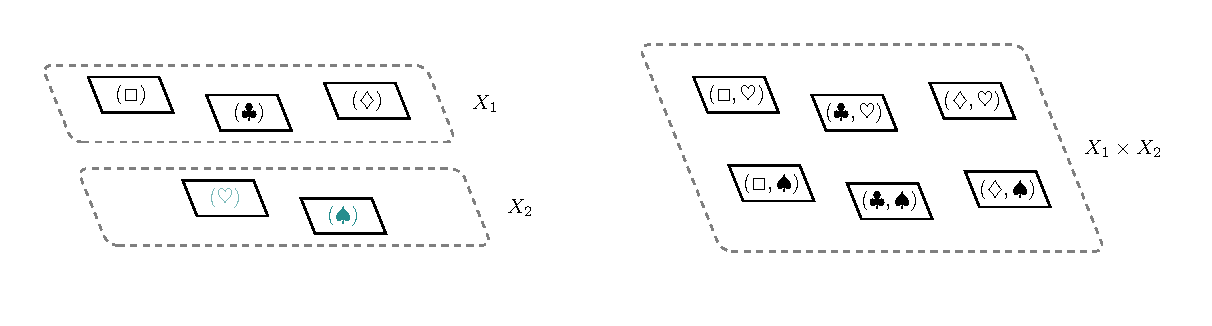
\includegraphics{figures/finite_product/X1X2/X1X2.pdf}

}

\subcaption{\label{fig-finite-product1}}

\end{minipage}%
%
\begin{minipage}{0.15\linewidth}
~\end{minipage}%
\newline
\begin{minipage}{0.15\linewidth}
~\end{minipage}%
%
\begin{minipage}{0.70\linewidth}

\centering{

\captionsetup{labelsep=none}\includegraphics{figures/finite_product/X2X1/X2x1.pdf}

}

\subcaption{\label{fig-finite-product2}}

\end{minipage}%
%
\begin{minipage}{0.15\linewidth}
~\end{minipage}%

\caption{\label{fig-finite-product}(a) The product set
\(X_{1} \times X_{2}\) consists of all ordered pairs combining one
element from \(X_{1}\) and one element from \(X_{2}\). (b) Reversing the
order of the pairs gives the product space \(X_{2} \times X_{1}\).}

\end{figure}%

By definition, each element of a binary product set is uniquely
specified by one element of \(X_{1}\) and one element of \(X_{2}\).
Consequently, every variable \(x\) taking values in the product set
\(X_{1} \times X_{2}\) can be represented by an ordered pair of
component variables, \[
x = (x_{1}, x_{2}),
\] with \(x_{1} \in X_{1}\) and \(x_{2} \times X_{2}\).

Again, order is important here. A variable \(x\) taking values in the
product set \(X_{2} \times X_{1}\) is instead comprised of the the
component variables \[
x = (x_{2}, x_{1}).
\]

\subsection{General Product Sets}\label{general-product-sets}

This construction immediately generalizes to any finite number of
component sets. Given \(I\) component sets indexed in a particular order
\[
\{ X_{1}, \ldots, X_{i}, \ldots X_{I} \},
\] we can construct a corresponding product set \[
X_{1} \times \ldots \times X_{i} \times \ldots \times X_{I}
=
\prod_{i = 1}^{I} X_{i}
\] from all of the ways that we can select one element from each
component set in that specified order, \[
( x_{1}, \ldots, x_{i}, \ldots, x_{I} )
\in \prod_{i = 1}^{I} X_{i}
\] with \(x_{i} \in X_{i}\). In other words, a variable taking values in
a finite product set is comprised of a \emph{sequence} of component
variables.

In theory, we could combine the component sets in any order. In
practice, however, it's easier to combine them in the order of their
indices, relabeling the indices if we ever need a different ordering.

Because product elements are specified by multiple component elements,
product sets are sometimes referred to as \textbf{multivariate} sets.
The component sets themselves are referred to in a variety of different
ways, including \textbf{degrees of freedom} and \textbf{coordinates}.

Conveniently, this construction generalizes immediately to a countably
infinite number of component sets: every element of a countably-infinite
product set is uniquely determined by an element from each of the
countably-infinite component sets. Defining product sets from an
uncountably infinite number of component sets requires just a little bit
more care. To ensure that choosing an uncountably infinite number of
elements at the same time is well-defined, we have to invoke the
infamous axiom of choice.

\subsection{Coordinating Indices}\label{coordinating-indices}

Many applications require working with multiple product variables at the
same time. A common strategy for differentiating between these different
variables is to label them with integer indices; for example we might
write \[
x_{1}, x_{2} \in \prod_{i = 1}^{I} X_{i}.
\] These indices, however, are easy to confuse with the indices used to
denote the component variables of which each product variable is
comprised.

In applications where indexing distinct product variables is useful, I
will use a comma to separate the two types of indices, with the first
index always labeling the different variables and the latter always
labeling the different components, \[
x_{j}
=
( x_{j, 1}, \ldots, x_{j, i}, \ldots, x_{j, I})
\in
\prod_{i = 1}^{I} X_{i}.
\] In other words, \(x_{j, i}\) refers to the \(i\)th component variable
of the \(j\)th product variable.

\subsection{Projection Functions}\label{projection-functions}

Conveniently, we can always recover the behavior of each the component
elements from a given product element. Consider, for example, the
component sets \(X_{1}\) and \(X_{2}\), the binary product space
\(X_{1} \times X_{2}\), and the product variable \(( x_{1}, x_{2} )\).

Ignoring the second component variable \(x_{2}\) leaves just \(x_{1}\),
which specifies a unique element of \(X_{1}\). In other words, each
element of \(X_{1} \times X_{2}\) defines a unique element of \(X_{1}\).
We can formalize this relationship as a function between the two sets,
\begin{alignat*}{6}
\varpi_{1} :\; & X_{1} \times X_{2} & &\rightarrow& \; & X_{1} &
\\
& (x_{1}, x_{2}) & &\mapsto& & x_{1} &.
\end{alignat*}

At the same time, ignoring the first component variable leaves
\(x_{2}\), which specifies a unique element of \(X_{2}\). This, in turn,
defines a relationship between \(X_{1} \times X_{2}\) and \(X_{1}\)
which we can encode in \emph{another} function, \begin{alignat*}{6}
\varpi_{2} :\; & X_{1} \times X_{2} & &\rightarrow& \; & X_{2} &
\\
& (x_{1}, x_{2}) & &\mapsto& & x_{2} &.
\end{alignat*}

More generally, ignoring all but one of the component variables in \[
( x_{1}, \ldots, x_{I} ) \in X^{1:I}
\] defines a map from the product set to the corresponding component
set, \begin{alignat*}{6}
\varpi_{i} :\; & \prod_{i = 1}^{I} X_{i} & &\rightarrow& \; & X_{i} &
\\
& (x_{1}, \ldots, x_{i}, \ldots, x_{I}) & &\mapsto& & x_{i} &.
\end{alignat*} Because these \(I\) functions \emph{project} the
composite product set to an individual component set, they are known as
\textbf{projection functions}. When the component sets are referred to
as ``coordinates'', the projection functions are also referred to as
\textbf{coordinate functions}.

Projection functions are useful for compactly organizing the composite
structure of product sets. We will be returning to them often.

\section{Thinned Product Sets}\label{thinned-product-sets}

The product set \(\prod_{i = 1}^{I} X_{i}\) is not the only product set
that we can construct from the component sets \[
\{ X_{1}, \ldots, X_{I} \}.
\] \emph{Any} selection of these component sets defines its own product
set.

More formally, any sequence of \(J \le I\) distinct component indices,
\[
\mathsf{i} = ( i_{1}, \ldots, i_{j}, \ldots, i_{J} )
\] with \[
i_{j} < i_{j + 1},
\] defines a product set \[
\prod_{i \in \mathsf{i} } X_{i}
=
\prod_{j = 1}^{J} X_{i_{j}}.
\] Each element of this product set is uniquely specified by an element
in each of the corresponding component sets, \[
( x_{i_{1}}, \ldots, x_{i_{J}} )
\in
\prod_{i \in \mathsf{i} } X_{i}
\] with \[
x_{i_{j}} \in X_{i_{j}}.
\] Because these product sets are comprised of only some of the
available component sets, I will refer to them as \textbf{thinned
product sets}.

There are many ways of selecting from the available component sets, and
hence many thinned product sets that we can construct in addition to the
full product set. In order to distinguishing between all of the
possibilities, especially when we are working with enough component sets
that explicit enumeration is unfeasible, we'll need to develop some
careful notation.

\subsection{Index Subsequences}\label{index-subsequences}

Given an initial sequence, we can construct \textbf{subsequences} by
removing some elements while maintaining the order of the remaining
elements. Using this terminology, the component indices that define each
thinned product set are subsequences of the sequence of all available
component indices, \[
(1, \ldots, i, \ldots, I).
\]

For example, from the initial sequence of component indices \[
( 1, 2, 3 )
\] we can construct six distinct, non-empty subsequences, \begin{align*}
&( 1 ), ( 2 ), ( 3 ),
\\
&( 1, 2 ), ( 1, 3 ), ( 2, 3 ).
\end{align*} The three atomic sequences identify one of the component
sets, but each of the three binary sequences defines a thinned product
set, \[
X_{1} \times X_{2}, \quad
X_{1} \times X_{3}, \quad
X_{2} \times X_{3}.
\]

I will denote the relationship between a sequence \(\mathsf{i}\) and a
subsequence \(\mathsf{i}'\) \[
\mathsf{i}' \, \vec{\subset} \, \mathsf{i}.
\] Here \(\subset\) communicates that the sequence on the left-hand side
contains fewer elements than the sequence on the right-hand side, while
the arrow communicates the consistent ordering.

Subsequences are basically subsets equipped with a persistent ordering.
It should be no surprise, then, that we can generalize all of the usual
subset operations to subsequences provided that we respect the ordering.

For example, we can define the intersection of two subsequences as the
elements shared by both sequences in the appropriate order. Starting
with the initial sequence \[
( 1, 2, 3, 4 ),
\] the intersection of the two subsequences \[
( 1, 2, 4 )
\] and \[
( 1, 3, 4 )
\] is the subsequence \[
(1, 4).
\] I will denote this ordered intersection as \[
( 1, 2, 4 ) \, \vec{\cap} \, (1, 3, 4) = (1, 4),
\] with the arrow once again communicating the consistent ordering of
subsequences.

Similarly, we can define an ordered union of two subsequences as the
appropriately ordered combination of their respective elements, \[
( 1, 3 ) \, \vec{\cup} \, ( 3, 4 )
=
( 1, 3, 4 ).
\]

These operations allow us to define a variety of useful manipulations of
a given sequence, such as partitions. Given an initial sequence
\(\mathsf{i}\), a \textbf{sequence partition} is a collection of \(K\)
subsequences \[
\mathsf{i}_{k} \, \vec{\subset} \, \mathsf{i}
\] that are nonempty \[
\mathsf{i}_{k} \ne (),
\] mutually disjoint, \[
\mathsf{i}_{k} \, \vec{\cap} \, \mathsf{i}_{k'} = ()
\] for \(k \ne k'\), and span the full sequence, \[
\vec{\cup}_{k = 1}^{K} \mathsf{i}_{k} = \mathsf{i}.
\]

\subsection{Multi-Index Notation}\label{multi-index-notation}

Given a collection of component sets, we can construct the full product
set as well as a myriad of thinned product sets. \textbf{Multi-index}
notation neatly organizes all of these possibilities by labeling each
product set with the corresponding sequence of component indices.

Specifically, we denote the thinned product set defined by the sequence
of component indices \[
\mathsf{i}
=
( i_{1}, \ldots, i_{J} ),
\] using a superscript, \[
X^{ \mathsf{i} }
\equiv
\prod_{i \in \mathsf{i} } X_{i}.
\] Similarly, we denote a variable taking values in this particular
thinned product set with a subscript, \[
x_{ \mathsf{i} } \in X^{\mathsf{i}}.
\]

The full product set built up from all available component indices is
used so often that it deserves its own special notation. If we denote
the sequence of all component indices by \[
1 \! : \! I = ( 1, \ldots, I ),
\] then we can denote the full product set as \[
X^{1:I}
=
\prod_{i \in 1:I} X_{i}
=
\prod_{i = 1}^{I} X_{i}.
\] Similarly, we can denote the corresponding product variable as \[
x_{1:I} \in X^{1:I}.
\]

Consider, for example, the component sets \(X_{1}\), \(X_{2}\),
\(X_{3}\), \(X_{4}\), and \(X_{5}\). Using multi-index notation we can
denote the full product set as \[
X_{1} \times X_{2} \times X_{3} \times X_{4} \times X_{5}
=
X^{1:5}
\] with product variables \[
x_{1:5} = ( x_{1}, x_{2}, x_{3}, x_{4}, x_{5} ).
\]

At the same time, if we select only the component indices \[
\mathsf{i} = ( 1, 3, 4 ),
\] then we can construct the thinned product set \[
X^{ \mathsf{i} }
=
X^{ (1, 3, 4) }
=
X_{1} \times X_{3} \times X_{4}
\] with product variables \[
x_{ \mathsf{i} }
=
x_{ (1, 3, 4) }
=
( x_{1}, x_{3}, x_{4} ).
\]

Multi-index notation is especially useful when working with multiple
product sets at the same time. For instance, let's return to our
previous example and then introduce another subsequence of component
indices, \[
\mathsf{i}' = ( 1, 2, 5 ).
\] We can now define three distinct product sets, \begin{align*}
& X_{1} \times X_{2} \times X_{3} \times X_{4} \times X_{5},
\\
& X_{1} \times X_{3} \times X_{4},
\\
& X_{1} \times X_{2} \times X_{5}.
\end{align*} Using multi-index notation, we can write out these product
spaces more compactly as \[
X^{1:5}, \quad
X^{ (1, 3, 4) }, \quad
X^{ (1, 2, 5) }.
\] This becomes even more compact if we use the names of the ordered
subsets of component indices, \[
X^{1:5}, \quad
X^{ \mathsf{i} }, \quad
X^{ \mathsf{i}' }.
\] Even with only the relatively small number of component spaces
available here, multi-index notation results in much more compact
equations.

The multi-index notation that I have defined here is a variant of the
multi-index notation popular in physics. This notation, however, is not
particularly common in probability theory or statistics. That said, I
will be using is extensively in this book.

\subsection{Generalized Projection
Functions}\label{generalized-projection-functions}

By dropping the unused component elements, any element of the full
product set defines an element of \emph{any} thinned product set. For
example, given the product element \[
( x_{1}, x_{2}, x_{3} ) \in X^{(1, 2, 3)},
\] we can define not only the component elements \[
x_{1} \in X_{1}, x_{2} \in X_{2}, x_{3} \in X_{3},
\] but also the thinned product elements \[
( x_{1}, x_{2}  ) \in X^{(1, 2)},
( x_{1}, x_{3}  ) \in X^{(1, 3)},
( x_{2}, x_{3}  ) \in X^{(2, 3)}.
\]

The relationship between full product elements and thinned product
elements defines generalized projection functions. Specifically, any
subsequence of component indices \[
\mathsf{i} \, \vec{\subset} \, 1:I,
\] defines a corresponding projection function \[
\varpi_{ \mathsf{i} } : X^{1:I} \rightarrow X^{ \mathsf{i} }.
\]

We can even construct projection functions between compatible thinned
product sets. If \[
\mathsf{i}' \; \vec{\subset} \; \mathsf{i}
\] then we can define the projection operators \[
\varpi_{ \mathsf{i'} }^{ \mathsf{i} } :
X^{ \mathsf{i} } \rightarrow X^{ \mathsf{i}' }.
\]

\section{Product Subsets}\label{product-subsets}

Just as an element in each of the component sets defines a unique
element from the corresponding product set, a subset in each of the
component sets defines a unique subset of the product set. Not every
subset of a product set, however, can be constructed in this way.

\subsection{Rectangles}\label{sec:rect}

Specifying a subset in each of the component sets, \[
\mathsf{x}_{i} \subseteq X_{i},
\] defines a unique subset of the product set, \[
\mathsf{x}_{1} \times \cdots \times
\mathsf{x}_{i} \times \cdots \times
\mathsf{x}_{I}
=
\times_{i = 1}^{I} \mathsf{x}_{i}
\subset
X^{1:I}.
\] The particular subsets of a product set of this form are known as
\textbf{product subsets}. We are, unfortunately, responsible for not
confusing these product subsets with arbitrary subsets of a product set.

Many of the important subsets of a product set can be constructed in
this way. The empty set of a product set, for example, is given by
combining the component empty sets, \[
\emptyset = \times_{i = 1}^{I} \emptyset_{i}.
\] Similarly, the full product set is given by combining the full
component sets, \[
X^{1:I} = \times_{i = 1}^{I} X_{i}.
\]

Not every subset of \(X^{1:I}\), however, is a product subset. More
formally, the product power set is \emph{not} the product of the
component power sets, \[
2^{ \prod_{i = 1}^{I} X_{i} }
\ne
\prod_{i = 1}^{I} 2^{X_{i}}.
\] In fact, the product power set is bigger than the product of the
component power sets, \[
2^{ \prod_{i = 1}^{I} X_{i} }
\supset
\prod_{i = 1}^{I} 2^{X_{i}}.
\] Typically the product power set is \emph{much} bigger than the
product of the component power set; in this case, most of subsets of the
product set are not product subsets!

On the product set \(\mathbb{R} \times \mathbb{R}\), the product of
finite intervals defines geometric rectangles
(Figure~\ref{fig-rectangle}). In analogy, more general product subsets
are often referred to as \textbf{rectangle subsets}, even when the
geometric intuition doesn't quite carry over. Despite the geometric
exaggeration, using ``rectangle'' instead of ``product subset'' is quite
useful for avoiding confusion between product subsets and more general
subsets of a product set.

\begin{figure}

\begin{minipage}{0.50\linewidth}

\centering{

\captionsetup{labelsep=none}
\includegraphics{figures/product_subset/r2_rectangle2/r2_rectangle.pdf}

}

\subcaption{\label{fig-rectangle1}}

\end{minipage}%
%
\begin{minipage}{0.50\linewidth}

\centering{

\captionsetup{labelsep=none}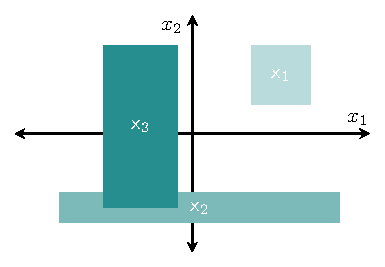
\includegraphics{figures/product_subset/r2_rectangle1/r2_rectangle.pdf}

}

\subcaption{\label{fig-rectangle2}}

\end{minipage}%

\caption{\label{fig-rectangle}(a) On the product set
\(\mathbb{R} \times \mathbb{R}\), geometric rectangles are defined by
the product two component interval subsets \(\mathsf{I}_{1}\) and
\(\mathsf{I}_{2}\). (b) Different component interval subsets result in a
diversity of rectangular shapes.}

\end{figure}%

\subsection{Cylinders}\label{sec:cyl}

Rectangle, however, is by no means the only geometric analogy that we
can abuse. Consider the product set \(S \times \mathbb{R}\). Here, the
product of a circle \(S\) and a linear interval
\(\mathsf{I} \subset \mathbb{R}\) defines a geometric cylinder
(Figure~\ref{fig-cylinder1}).

Analogizing this geometry motivates a class of subsets on \emph{any}
product set. A \textbf{generalized cylinder subset}, or just
\textbf{cylinder subset} for short, is defined to be a rectangle subset
where all but a \emph{finite number} of component subsets equals the
full component set (Figure~\ref{fig-cylinder2}).

\begin{figure}

\begin{minipage}{0.15\linewidth}
~\end{minipage}%
%
\begin{minipage}{0.35\linewidth}

\centering{

\captionsetup{labelsep=none}
\includegraphics{figures/product_subset/cylinder_rectangle/cylinder.pdf}

}

\subcaption{\label{fig-cylinder1}}

\end{minipage}%
%
\begin{minipage}{0.35\linewidth}

\centering{

\captionsetup{labelsep=none}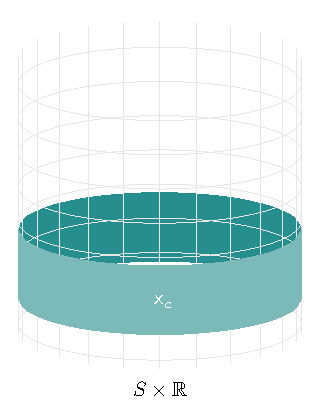
\includegraphics{figures/product_subset/cylinder_cylinder/cylinder.pdf}

}

\subcaption{\label{fig-cylinder2}}

\end{minipage}%
%
\begin{minipage}{0.15\linewidth}
~\end{minipage}%

\caption{\label{fig-cylinder}(a) On the product set
\(S \times \mathbb{R}\), geometric rectangles, such as
\(\mathsf{x}_{r}\), are defined by products of angular intervals
\(\mathsf{I}_{2} \subset S\) and linear intervals
\(\mathsf{I}_{1} \subset \mathbb{R}\). (b) Geometric cylinders, such as
\(\mathsf{x}_{c}\), are a special case where the angular interval covers
all of \(S\). The term ``cylinder subset'' is used more generally for
any product subset where all but a finite number of component subsets
equal the full component set.}

\end{figure}%

Note that, by this definition, there is no strict difference between
rectangle subsets and cylinder subsets on a product set with only a
finite number of component sets. The distinction, however, becomes
critical when considering product sets built up from an infinite number
of component sets. Here, cylinder subsets ensure that only a finite
number of components are actively contributing to the behavior of the
product subset at any given time.

\subsection{Cross Sections}\label{sec:cross}

When the component subsets are either full or atomic, with at least one
component subset atomic, the resulting cylinder subset on the product
space is known as a \textbf{cross section}. Cross sections model the
behavior of a product set when we bind some, but not all, of the
component sets to particular elements.

\begin{figure}

\begin{minipage}{0.50\linewidth}

\centering{

\captionsetup{labelsep=none}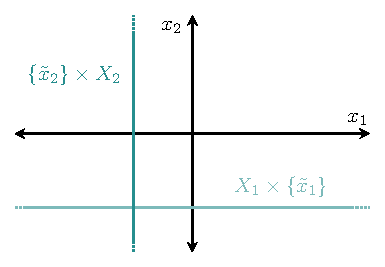
\includegraphics{figures/product_subset/r2_cross/r2_cross.pdf}

}

\subcaption{\label{fig-cross1}}

\end{minipage}%
%
\begin{minipage}{0.07\linewidth}
~\end{minipage}%
%
\begin{minipage}{0.35\linewidth}

\centering{

\captionsetup{labelsep=none}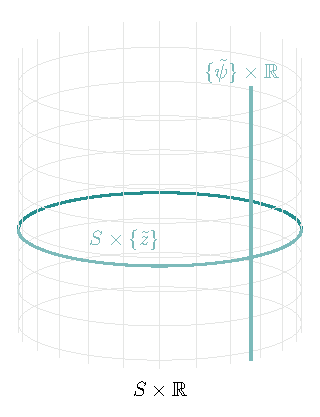
\includegraphics{figures/product_subset/cylinder_cross/cylinder_cross.pdf}

}

\subcaption{\label{fig-cross2}}

\end{minipage}%
%
\begin{minipage}{0.07\linewidth}
~\end{minipage}%

\caption{\label{fig-cross}Cross sections are a special type of cylinder
subset where each component subset is either full or atomic, and at
least one is atomic. (a) On the product set
\(\mathbb{R} \times \mathbb{R}\), cross sections trace out vertical and
horizontal lines, and (b) on the product set \(S \times \mathbb{R}\)
cross sections trace out circles and vertical lines.}

\end{figure}%

For instance, binding \(\tilde{x}_{1} \in X_{1}\) doesn't specify a
point in the cross section \(X_{1} \times X_{2}\). It does, however,
restrict the possibilities to the cross section \[
\{ \tilde{x}_{1} \} \times X_{2} \subset X_{1} \times X_{2}.
\] Similarly, fixing \(\tilde{x}_{2} \in X_{2}\) restricts the product
set to the cross section \[
X_{1} \times \{ \tilde{x}_{2} \} \subset X_{1} \times X_{2}.
\] More generally, binding the component elements \[
\{ \tilde{x}_{i} \mid i \in \mathsf{i} \}
\] for \[
\mathsf{i} \, \vec{\subset} \, 1:I,
\] but leaving the complementary component elements \[
\{ x_{i} \mid i \in \mathsf{i}^{c} \}
\] free, defines a cross section of the product set \(X^{1:I}\).

The most awkward aspect of cross sections is compactly denoting which
components have been constrained. I will often write cross sections
symbolically as \[
X^{ \mathsf{i}^{c} } \times \{ x_{ \mathsf{i} } \}
\subset X^{1:I},
\] with the understanding that the component objects have to be
reordered as necessary. If, for example, \(I = 5\) and
\(\mathsf{i} = (2, 4)\), then \begin{align*}
X^{ \mathsf{i}^{c} } \times \{ x_{ \mathsf{i} } \}
&=
X^{ (1, 3, 5) } \times \{ x_{ (2, 4) } \}
\\
&=
X_{1} \times \{ x_{2} \} \times
X_{3} \times \{ x_{4} \} \times X_{5}.
\end{align*}

Cross sections can also be written in terms of projection functions.
Specifically, each level set of the projection function \[
\varpi_{ \mathsf{i} } : X^{1:I} \rightarrow X^{ \mathsf{i} }
\] defines a unique cross section, \[
\varpi_{ \mathsf{i} }^{-1} ( \tilde{x}_{ \mathsf{i} } )
=
X^{ \mathsf{i}^{c} } \times \{ \tilde{x}_{ \mathsf{i} } \}.
\]

Once we bind the component elements \[
\{ \tilde{x}_{i} \mid i \in \mathsf{i} \},
\] an element of the full product set is uniquely determined by any
configuration of the remaining component elements \[
\{ x_{i} \mid i \in \mathsf{i}^{c} \}.
\] Consequently, these complementary component elements specify elements
of the cross section \[
X^{ \mathsf{i}^{c} } \times \{ \tilde{x}_{ \mathsf{i} } \}
\subset X^{1:I}.
\] These elements, however, also define an element of the thinned
product set \(X^{ \mathsf{i}^{c} }\).

In other words, every element of a cross section is uniquely identified
with an element of the corresponding thinned product set. More formally,
we have a natural bijection between the two, \[
X^{ \mathsf{i}^{c} } \times \{ x_{ \mathsf{i} } \}
\cong
X^{ \mathsf{i}^{c} }.
\] More intuitively, we can always interpret the cross sections
\(X^{ \mathsf{i}^{c} } \times \{ x_{ \mathsf{i} } \}\) as distinct
copies of \(X^{ \mathsf{i}^{c} }\), each of which is distinguished by an
element of the thinned product set \[
x_{ \mathsf{i} } \in X^{ \mathsf{i} }.
\]

The cross sections \[
X_{1} \times X_{2} \times \{ x_{3} \}
\subset
X_{1} \times X_{2} \times X_{3},
\] for instance, each behave like a copy of the thinned product set \[
X_{1} \times X_{2}.
\] Once we've fixed \(x_{3} \in X_{3}\), any element of the resulting
cross section defines a corresponding element of the thinned product and
vice versa. This allows us to jump between a more global perspective --
cross sections as subsets of the full product set -- and a more local
perspective -- thinned product sets -- at our convenience.

While each cross section can be identified with a common thinned product
set, the \emph{behavior} within each cross section at any given time
can, in general, be different. Consequentially, we have to be careful to
respect the individuality of each cross section.

\subsection{Rectangular Subset
Operations}\label{rectangular-subset-operations}

Most of the subset operations are not compatible with the composite
structure of a rectangle subset.

The complement of a rectangle subset, for example, is not generally
given by applying the complement operation to each of the component
subsets (Figure~\ref{fig-product-set-complement}), \[
\mathsf{x}^{c} \ne \times_{i = 1}^{I} \mathsf{x}_{i}^{c}.
\] Instead the product of the \(\mathsf{x}_{i}^{c}\) typically includes
fewer elements than the complement of the product of the
\(\mathsf{x}_{i}^{c}\), \[
\times_{i = 1}^{I} \mathsf{x}_{i}^{c}
\subseteq
\left(
\times_{i = 1}^{I} \mathsf{x}_{i}
\right)^{c}.
\]

\begin{figure}

\begin{minipage}{0.25\linewidth}
~\end{minipage}%
%
\begin{minipage}{0.50\linewidth}

\centering{

\captionsetup{labelsep=none}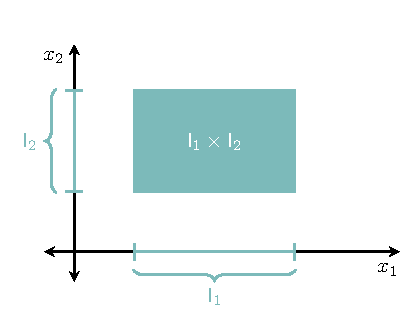
\includegraphics{figures/product_subset_complement/1/rectangles.pdf}

}

\subcaption{\label{fig-psc1}}

\end{minipage}%
%
\begin{minipage}{0.25\linewidth}
~\end{minipage}%
\newline
\begin{minipage}{0.50\linewidth}

\centering{

\captionsetup{labelsep=none}
\includegraphics{figures/product_subset_complement/2/rectangles.pdf}

}

\subcaption{\label{fig-psc2}}

\end{minipage}%
%
\begin{minipage}{0.50\linewidth}

\centering{

\captionsetup{labelsep=none}
\includegraphics{figures/product_subset_complement/3/rectangles.pdf}

}

\subcaption{\label{fig-psc3}}

\end{minipage}%

\caption{\label{fig-product-set-complement}(a) The construction of a
rectangle subset from component subsets doesn't commute with the
complement operator. (b) Taking the product first and then applying the
complement operator typically doesn't result in another rectangular
subset (c). Applying the complement operator to each component subset
and then taking their product, however, does.}

\end{figure}%

Similarly, the union of two rectangle subsets, \[
\mathsf{x} = \times_{i = 1}^{I} \mathsf{x}_{i}
\] and \[
\mathsf{x}' = \times_{i = 1}^{I} \mathsf{x}'_{i},
\] is not generally given by the product of the component unions
(Figure~\ref{fig-product-set-union}), \[
\mathsf{x} \cup \mathsf{x}'
\ne
\times_{i = 1}^{I} \mathsf{x}_{i} \cup \mathsf{x}'_{i}.
\] In general, the product of the component unions is not a rectangle
subset. Moreover, it it larger than the union of the products, \[
\mathsf{x} \cup \mathsf{x}'
\subseteq
\times_{i = 1}^{I} \mathsf{x}_{i} \cup \mathsf{x}_{i'}.
\]

\begin{figure}

\begin{minipage}{0.25\linewidth}
~\end{minipage}%
%
\begin{minipage}{0.50\linewidth}

\centering{

\captionsetup{labelsep=none}
\includegraphics{figures/product_subset_union/1/rectangles.pdf}

}

\subcaption{\label{fig-psu1}}

\end{minipage}%
%
\begin{minipage}{0.25\linewidth}
~\end{minipage}%
\newline
\begin{minipage}{0.50\linewidth}

\centering{

\captionsetup{labelsep=none}
\includegraphics{figures/product_subset_union/2/rectangles.pdf}

}

\subcaption{\label{fig-psu2}}

\end{minipage}%
%
\begin{minipage}{0.50\linewidth}

\centering{

\captionsetup{labelsep=none}
\includegraphics{figures/product_subset_union/3/rectangles.pdf}

}

\subcaption{\label{fig-psu3}}

\end{minipage}%

\caption{\label{fig-product-set-union}The union operator also doesn't
commute with (a) the construction of rectangle subsets. (b) Taking the
product first and then applying the union operator usually results in a
non-rectangle subset that is smaller (c) than the rectangular subset
given by applying the union operator to each component subset and then
taking their product.}

\end{figure}%

The lone exception is the intersection of rectangle subsets, which can
always be derived from the intersection of the component subsets
(Figure~\ref{fig-product-set-intersection}), \[
\mathsf{x} \cap \mathsf{x}'
=
\times_{i = 1}^{I} \mathsf{x}_{i} \cap \mathsf{x}'_{i}.
\]

\begin{figure}

\begin{minipage}{0.25\linewidth}
~\end{minipage}%
%
\begin{minipage}{0.50\linewidth}

\centering{

\captionsetup{labelsep=none}
\includegraphics{figures/product_subset_intersection/1/rectangles.pdf}

}

\subcaption{\label{fig-psi1}}

\end{minipage}%
%
\begin{minipage}{0.25\linewidth}
~\end{minipage}%
\newline
\begin{minipage}{0.50\linewidth}

\centering{

\captionsetup{labelsep=none}
\includegraphics{figures/product_subset_intersection/2/rectangles.pdf}

}

\subcaption{\label{fig-psi2}}

\end{minipage}%
%
\begin{minipage}{0.50\linewidth}

\centering{

\captionsetup{labelsep=none}
\includegraphics{figures/product_subset_intersection/3/rectangles.pdf}

}

\subcaption{\label{fig-psi3}}

\end{minipage}%

\caption{\label{fig-product-set-intersection}Of the three subset
operators, only the intersection operator commutes with (a) the
construction of rectangle subsets. (b) Taking the product first and then
applying the intersection operator always gives the same rectangle
subset as (c) applying the intersection operator to each component
subset and then taking their product.}

\end{figure}%

An immediate consequence of these properties is that rectangle subsets
are closed under intersections but not unions and complements. While
closure is often useful in practice, in this case the lack of closure is
actually quite useful. In particular, it allows us to build up
non-rectangle subsets by applying set operations to rectangle subsets.
We'll come back to this point in \hyperref[sec:topology]{Section 5.4}.

\section{Decomposing Product Sets}\label{sec:decomposition}

The composite structure of product sets allows us to slice and dice them
into smaller pieces. Because the smaller pieces are often easier to
directly manipulate, these decompositions can be extremely useful in
practical applications.

\subsection{Two Component Sets}\label{two-component-sets}

Let's start as simply as possibly by considering the two component sets
\(X_{1}\) and \(X_{2}\) and their product \(X_{1} \times X_{2}\).

\subsubsection{Decomposition}\label{decomposition}

Decomposing \(X_{1}\) into the union of its atomic subsets, \[
X_{1} = \bigcup_{ x_{1} \in X_{1} } x_{i},
\] induces a similar decomposition of the product set into a union of
cross sections, (Figure~\ref{fig-decomp-2d-1}), \begin{align*}
X_{1} \times X_{2}
&=
\left( \bigcup_{ x_{1} \in X_{1} } \{ x_{i} \} \right)
\times X_{2}
\\
&=
\bigcup_{ x_{1} \in X_{1} }
\left( \{ x_{1} \} \times X_{2} \right).
\end{align*} Because these cross sections can be interpreted as copies
of \(X_{2}\), we can interpret this as a decomposition of the product
set into repeated instances that component set.

\begin{figure}

\begin{minipage}{0.15\linewidth}
~\end{minipage}%
%
\begin{minipage}{0.70\linewidth}

\centering{

\captionsetup{labelsep=none}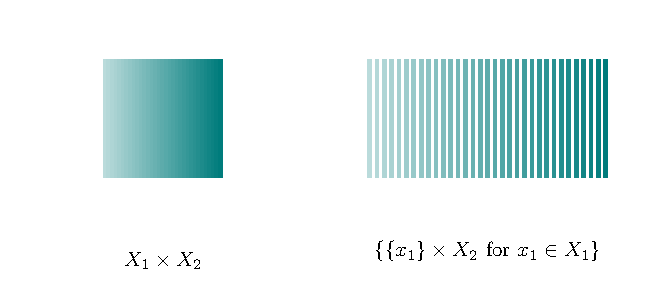
\includegraphics{figures/decomposition/2d/X1/X1.pdf}

}

\subcaption{\label{fig-decomp-2d-1}}

\end{minipage}%
%
\begin{minipage}{0.15\linewidth}
~\end{minipage}%
\newline
\begin{minipage}{0.15\linewidth}
~\end{minipage}%
%
\begin{minipage}{0.70\linewidth}

\centering{

\captionsetup{labelsep=none}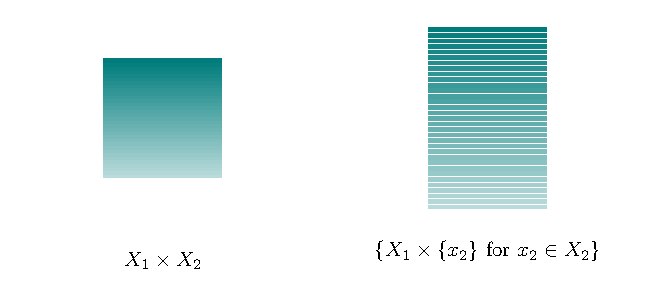
\includegraphics{figures/decomposition/2d/X2/X2.pdf}

}

\subcaption{\label{fig-decomp-2d-2}}

\end{minipage}%
%
\begin{minipage}{0.15\linewidth}
~\end{minipage}%

\caption{\label{fig-fig-decomp-2d}(a) When we decompose \(X_{1}\) into
atomic subsets, the product set \(X_{1} \times X_{2}\) decomposes into a
union of cross sections, \(\{ x_{1} \} \times X_{2}\), each of which
behaves like a replication of the component set \(X_{1}\). (b) The
product set can also be sliced in the other direction, resulting in the
cross sections \(X_{1} \times \{ x_{2} \}\).}

\end{figure}%

This procedure can also be applied to the second component set,
resulting in the decomposition (Figure~\ref{fig-decomp-2d-2}) \[
X_{1} \times X_{2}
=
\bigcup_{ x_{2} \in X_{2} }
\left( X_{1} \times \{ x_{2} \} \right).
\] Binary product spaces can be sliced in either direction!

\subsubsection{Composition}\label{composition}

Cross sections can also be used to construct product sets in the first
place. Consider, for instance, starting with only the component set
\(X_{1}\). Introducing a copy of \(X_{2}\) for each \(x_{1} \in X_{1}\)
defines the cross sections \(\{ x_{1} \} \times X_{2}\), and the union
of these cross sections is exactly the product set
\(X_{1} \times X_{2}\). Equivalently, if we start with \(X_{2}\) then we
can construct \(X_{1} \times X_{2}\) by introducing a copy of \(X_{1}\)
for each \(x_{2} \in X_{2}\).

Indeed, this construction is basically how ordered pairs are formally
defined in the first place. In abstract set theory, an ordered pair is
defined by an element from one of the component sets and a compatible,
unordered pair of component elements, \[
( x_{1}, x_{2} ) \equiv \{ x_{1}, \{ x_{1}, x_{2} \} \}
\] or \[
( x_{1}, x_{2} ) \equiv \{ x_{2}, \{ x_{1}, x_{2} \} \}.
\] Given the initial component element, the compatible component
pairings effectively defines a cross section.

\subsubsection{Sequential Specification}\label{sequential-specification}

These procedures offers some geometric insight into how we
\emph{sequentially} specify elements of a product set. Selecting a
component element \[
\tilde{x}_{1} \in X_{1}
\] doesn't fully determine an element from the product set. It does,
however, restrict the possibilities to the cross section \[
\{ \tilde{x}_{1} \} \times X_{2} \subset X_{1} \times X_{2}.
\] To completely determine a product element, we need to select product
element from the corresponding cross section
(Figure~\ref{fig-seq-sel-2d-12}) \[
\tilde{x} \in \{ \tilde{x}_{1} \} \times X_{2}.
\]

Alternatively, we can select an element from the second component set,
\[
\tilde{x}_{2} \in X_{2},
\] and then an element from the cross section
(Figure~\ref{fig-seq-sel-2d-21}), \[
\tilde{x} \in X_{1} \times \{ \tilde{x}_{2} \}.
\]

\begin{figure}

\begin{minipage}{\linewidth}

\centering{

\captionsetup{labelsep=none}
\includegraphics{figures/sequential_selection/2d/X1X2/X1X2.pdf}

}

\subcaption{\label{fig-seq-sel-2d-12}}

\end{minipage}%
\newline
\begin{minipage}{\linewidth}

\centering{

\captionsetup{labelsep=none}
\includegraphics{figures/sequential_selection/2d/X2X1/X2X1.pdf}

}

\subcaption{\label{fig-seq-sel-2d-21}}

\end{minipage}%

\caption{\label{fig-seq-sel}A product set element
\((\tilde{x}_{1}, \tilde{x}_{2}) \in X_{1} \times X_{2}\) can be
sequentially constructed in two different ways. (a) Selecting
\(\tilde{x}_{1} \in X_{1}\) restricts the possible elements to the cross
section \(\{ \tilde{x}_{1} \} \times X_{2}\). (b) Alternatively, we can
first select \(\tilde{x}_{2} \in X_{2}\) before selecting a point from
the corresponding cross section,
\(\tilde{x}_{1} \in X_{1} \times \{ \tilde{x}_{2} \}\). Either way, we
don't have to consider the product set in its entirely.}

\end{figure}%

\subsection{Three Component Sets}\label{three-component-sets}

Increasing the number of component sets dramatically increases the ways
that we can slice and dice the resulting product set. Before jumping in
more generally, let's see what happens when we consider just one more
component set to bring us to \(X_{1}\), \(X_{2}\), and \(X_{3}\).

\subsubsection{Decomposition Into Binary Product
Sets}\label{decomposition-into-binary-product-sets}

Expanding the first component set into its atomic subsets induces the
cross section decomposition \[
X_{1} \times X_{2} \times X_{3}
=
\bigcup_{ x_{1} \in X_{1} }
\{ x_{1} \} \times X_{2} \times X_{3}.
\] In this case, the product set decomposes into replications of the
binary product set \(X_{2} \times X_{3}\).

At the same time, expanding the other two component sets gives the
alternative decompositions (Figure~\ref{fig-decomp-3d-1}) \[
X_{1} \times X_{2} \times X_{3}
=
\bigcup_{ x_{1} \in X_{1} }
\{ x_{1} \} \times X_{2} \times X_{3}
\] and \[
X_{1} \times X_{2} \in X_{3}
=
\bigcup_{ x_{3} \in X_{3} }
X_{1} \times X_{2} \times \{ x_{3} \}.
\]

\begin{figure}

\centering{


\includegraphics[width=1\textwidth,height=\textheight]{figures/decomposition/3d/1/1.pdf}

}

\caption{\label{fig-decomp-3d-1}Isolating any one of its component sets
decomposes the product set \(X_{1} \times X_{2} \times X_{3}\) into
replications of binary product sets. Slicing along \(X_{1}\), for
example, decomposes the product set into the cross sections
\(\{ x_{1} \} \times X_{2} \times X_{3}\), each of which can be treated
as a distinct copy of \(X_{2} \times X_{3}\).}

\end{figure}%

\subsubsection{Decomposition Into Component
Sets}\label{decomposition-into-component-sets}

We can also expanding binary products of component sets into atomic
subsets. This yields three more decompositions of the full product set
(Figure~\ref{fig-decomp-3d-2}), \begin{align*}
X_{1} \times X_{2} \times X_{3}
&=
\bigcup_{ (x_{1}, x_{2}) \in X_{1} \times X_{2} }
\{ x_{1} \} \times \{ x_{2} \} \times X_{3}
\\
X_{1} \times X_{2} \times X_{3}
&=
\bigcup_{ (x_{1}, x_{3}) \in X_{1} \times X_{3} }
\{ x_{1} \} \times X_{2} \times \{ x_{3} \}
\\
X_{1} \times X_{2} \times X_{3}
&=
\bigcup_{ (x_{2}, x_{3}) \in X_{2} \times X_{3} }
X_{1} \times \{ x_{2} \} \times \{ x_{3} \}.
\end{align*} We can slice three-component product sets into not only
binary product sets but also individual component sets!

\begin{figure}

\centering{


\includegraphics[width=1\textwidth,height=\textheight]{figures/decomposition/3d/2/2.pdf}

}

\caption{\label{fig-decomp-3d-2}Isolating two of its component sets at
the same time decomposes the product set
\(X_{1} \times X_{2} \times X_{3}\) into replications of the single,
remaining component set. Jointly slicing along \(X_{1}\) and \(X_{2}\),
for example, dices the product set into the cross sections
\(\{ x_{1} \} \times \{ x_{2} \} \times X_{3}\), each of which can be
treated as a distinct copy of \(X_{3}\).}

\end{figure}%

\subsubsection{Recursive Decomposition}\label{recursive-decomposition}

Some of these decompositions can be further \emph{refined}. Consider,
for instance, the decomposition \[
X_{1} \times X_{2} \times X_{3}
=
\bigcup_{ (x_{1}, x_{2}) \in X_{1} \times X_{2} }
\{ x_{1} \} \times \{ x_{2} \} \times X_{3}.
\] The set that indexes each copy of \(X_{3}\) can be further decomposed
into \[
X_{1} \times X_{2}
=
\bigcup_{ x_{1} \in X_{1} }
\{ x_{1} \} \times X_{2}.
\] This is equivalent to decomposing the full product set into \[
\bigcup_{ x_{1} \in X_{1} }
\bigcup_{ x_{2} \in \{ x_{1} \} \times X_{2} }
\{ x_{1} \} \times \{ x_{2} \} \times X_{3}.
\]

Equivalently, we can decompose \(X_{1} \times X_{2}\) into \[
X_{1} \times X_{2}
=
\bigcup_{ x_{2} \in X_{2} }
X_{1} \times \{ x_{2} \},
\] which decomposes the full product set into \[
\bigcup_{ x_{2} \in X_{2} }
\bigcup_{ x_{1} \in X_{1} \times \{ x_{2} \} }
\{ x_{1} \} \times \{ x_{2} \} \times X_{3}.
\]

\subsubsection{Composition}\label{composition-1}

Each of these decompositions motivates a different way to sequential
construct a product set.

For example, we can lift \(X_{1}\) to
\(X_{1} \times X_{2} \times X_{3}\) by introducing a copy of
\(X_{2} \times X_{3}\) for each element \(x_{1} \times X_{1}\).
Alternatively, we can start with \(X_{2}\) and introduce copies of
\(X_{1} \times X_{3}\) or start with \(X_{3}\) and introduce copies of
\(X_{1} \times X_{2}\).

At the same time, if we start with \(X_{1} \times X_{2}\) then we can
construct \(X_{1} \times X_{2} \times X_{3}\) by introducing a copy of
the third component set \(X_{3}\) for each ordered pair
\((x_{2}, x_{3}) \in X_{1} \times X_{2}\). Starting with
\(X_{1} \times X_{3}\) or \(X_{1} \times X_{2}\) requires replicating
\(X_{2}\) or \(X_{1}\), respectively.

Finally, we can build up the full product set from smaller pieces using
more steps. We could, for instance, start with \(X_{1}\) and then
introduce a copy of \(X_{2}\) for each initial element to define
\(X_{1} \times X_{2}\). At this point, we can replicate \(X_{3}\) for
each ordered pair \((x_{2}, x_{3}) \in X_{1} \times X_{2}\). Each
permutation of the component indices defines a unique construction path.

\subsubsection{Sequentially Specifying Product
Elements}\label{sequentially-specifying-product-elements}

Once again, these decompositions offer geometric insight into what is
happening as we sequentially specify elements of the full product set.
For example, we might specify an element of the first component set, \[
\tilde{x}_{1} \in X_{1}
\] and then an element of the cross section \[
\tilde{x} \in \{ x_{1} \} \times X_{2} \times X_{3}.
\] In practice, this is equivalent to selecting \(x_{1}\) and then
\(x_{2}\) and \(x_{3}\) at the same time.

Alternatively, we might start by specifying the pair \[
(\tilde{x}_{1}, \tilde{x}_{2}) \in X_{1} \times X_{2}
\] before selecting from the cross section \[
\tilde{x} \in \{ x_{1} \} \times \{ x_{2} \} \times X_{3}.
\] This is equivalent to selecting \(x_{1}\) and \(x_{2}\) at the same
time and then selecting \(x_{3}\).

We might also specify component elements one at a time
(Figure~\ref{fig-seq-sel-3d}), starting with \[
\tilde{x}_{1} \in X_{1},
\] then \[
\tilde{x}_{2} \in \{ \tilde{x}_{1} \} \times X_{2},
\] and finally \[
\tilde{x}
\in
\{ x_{1} \} \times \{ x_{2} \} \times X_{3}
\subset
\{ \tilde{x}_{1} \} \times X_{2}
\] In practice, this corresponds to selecting \(x_{1}\) before \(x_{2}\)
and then lastly \(x_{3}\).

\begin{figure}

\centering{

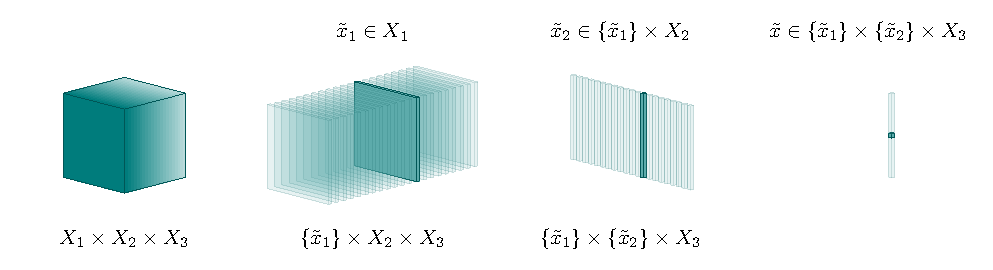
\includegraphics[width=1\textwidth,height=\textheight]{figures/sequential_selection/3d/3d.pdf}

}

\caption{\label{fig-seq-sel-3d}Specifying component elements one by one
builds up an element of the product set sequentially. For instance,
taking \(\tilde{x}_{1} \in X_{1}\) restricts the possible elements to
the cross section \(\{ \tilde{x}_{1} \} \times X_{2} \times X_{3}\). At
this point, selecting an element \(\tilde{x}_{2} \in X_{2}\) restricts
this cross section to the more refined cross section
\(\{ x_{1} \} \times \{ x_{2} \} \times X_{3}\). Finally, taking
\(\tilde{x}_{3} \in X_{3}\) selects a product set element from this
cross section.}

\end{figure}%

Across the last three examples, I have maintained the same order of the
component sets. More generally, however, we can consider the component
sets in any order. For example, \begin{align*}
\tilde{x}_{2} &\in X_{2}
\\
\tilde{x} &\in X_{1} \times \{ x_{2} \} \times X_{3},
\end{align*} \begin{align*}
(\tilde{x}_{2}, \tilde{x}_{3}) &\in X_{2} \times X_{3}
\\
\tilde{x} &\in X_{1} \times \{ x_{2} \} \times \{ x_{3} \},
\end{align*} and \begin{align*}
\tilde{x}_{2} &\in X_{2}
\\
\tilde{x}_{3} &\in \{ \tilde{x}_{2} \} \times X_{3}
\\
\tilde{x} &\in X_{1} \times \{ x_{2} \} \times \{ x_{3} \}
\end{align*} are all valid, but by no means exhaustive, ways to build up
an element of a product set.

\subsection{General Case}\label{general-case}

Once we go beyond a few component sets, the number of ways that we can
decompose of the resulting product set is so large that the
possibilities can be overwhelming. Fortunately, multi-index notation
makes it straightforward to specify any particular decomposition.

\subsubsection{Direct Decomposition and
Composition}\label{direct-decomposition-and-composition}

Given a subsequence of component indices, \[
\mathsf{i} \, \vec{\subset} \, 1:I,
\] we can define three product sets: the full product set, \(X^{1:I}\),
and two thinned product sets, \(X^{ \mathsf{i} }\) and
\(X^{ \mathsf{i}^{c} }\).

Decomposing the thinned product set \(X^{ \mathsf{i} }\) into its atomic
elements, \[
X^{ \mathsf{i} }
=
\bigcup_{ x_{ \mathsf{i} } \in X^{ \mathsf{i} } }
\{ x_{ \mathsf{i} } \},
\] decomposes the full product set into the corresponding cross
sections, \[
X^{1:I}
=
\bigcup_{ x_{ \mathsf{i} } \in X^{ \mathsf{i} } }
X_{ \mathsf{i}^{c} }\times \{ x_{ \mathsf{i} } \}.
\]

At the same time, replicating \(X^{ \mathsf{i}^{c} }\) for each element
of \(X^{ \mathsf{i} }\) lifts \(X^{ \mathsf{i} }\) into the full product
set \(X^{1:I}\). Heuristically, we can write this composition as \[
x = ( x_{ \mathsf{i} }, x_{ \mathsf{i}^{c} } ),
\] with the understanding that the component elements must be reordered
as necessary.

For example, if \(I = 5\) and \(\mathsf{i} = (2, 4)\), then we would
first select an element \[
x_{ (2, 4) } \in X^{ (2, 4) }
\] before selecting an element of \[
x_{ (1, 3, 5) } \in X^{ (1, 3, 5) }.
\] We could then write the resulting product set element as
\begin{align*}
x
&=
( x_{ (2, 4) }, x_{ (1, 3, 5) }  )
\\
&=
( (x_{2}, x_{4}), ( x_{1}, x_{3}, x_{5}) )
\\
&=
( x_{1}, x_{2}, x_{3}, x_{4}, x_{5} ).
\end{align*}

\subsubsection{Recursive Decomposition and
Composition}\label{recursive-decomposition-and-composition}

Decomposing \(X^{1:I}\) into the cross sections \[
\bigcup_{ x_{ \mathsf{i} } \in X^{ \mathsf{i} } }
X_{ \mathsf{i}^{c} }\times \{ x_{ \mathsf{i} } \}
\] can be impractical if the thinned product space \(X^{ \mathsf{i} }\)
is still too overwhelming. Fortunately, nothing is stopping us from
decomposing this space int more manageable pieces.

In particular, the subsequence of component indices \[
\mathsf{i}' \, \vec{\subset} \, \mathsf{i}
\] decomposes \(X^{ \mathsf{i} }\) into cross sections, \[
X^{ \mathsf{i} }
=
\bigcup_{ x_{ \mathsf{i}' } \in X^{ \mathsf{i}' }  }
X^{ \mathsf{i} \setminus \mathsf{i}' } \times
\{ x_{ \mathsf{i}' } \}.
\] If, at this point, the thinner product \(X^{ \mathsf{i}' }\) is still
too much to handle, then we can iterate until we've broken the system
down into sufficiently manageable pieces.

There are many ways that this recursive decomposition could proceed.
Conveniently, each possibility is completely determined by a partition
of the component indices \(1:I\) into disjoint subsequences \[
( \mathsf{i}_{1}, \ldots, \mathsf{i}_{K} )
\] with \[
\mathsf{i}_{k} \, \vec{\subset} \, 1:I.
\]

First, we iteratively remove the component indices in each
\(\mathsf{i}_{k}\) to define a sequence of thinning product sets,
\(X^{ \mathsf{j}_{k} }\) with \[
\mathsf{j}_{k}
=
\vec{\cup}_{k' = k}^{K} \mathsf{i}_{k'}.
\] Next, we decompose the full product set into copies of
\(X^{ \mathsf{i}_{1} }\), \[
X^{1:I}
=
\bigcup_{ x_{ \mathsf{j}_{2} } \in X^{ \mathsf{j}_{2} } }
X^{ \mathsf{i}_{1} } \times \{ x_{ \mathsf{j}_{2} }  \}.
\] At this point we can iterate \(K - 2\) more times, decomposing
\(X^{ \mathsf{j}_{k} }\) into copies of \(X^{ \mathsf{i}_{k} }\), \[
X^{ \mathsf{j}_{k} }
=
\bigcup_{ x_{ \mathsf{j}_{k + 1} } \in X^{ \mathsf{j}_{k + 1} } }
X^{ \mathsf{i}_{k} } \times \{ x_{ \mathsf{j}_{k + 1} }  \}.
\] Each iteration peels off the component sets whose indices are in
\(\mathsf{i}_{k}\).

Working through this subsequence partition backwards also allows us to
construct the full product set in \(K - 1\) total steps. Starting with
\(k = K\), each iteration lifts the thinned product set
\(X^{ \mathsf{j}_{k} }\) into the slightly less-thinned product set
\(X^{ \mathsf{j}_{k - 1} }\) by replicating
\(X^{ \mathsf{i}_{k - 1} }\).

For a concrete demonstration, consider \(I = 7\) and the sequence
partition \[
( \mathsf{i}_{1} = (2, 4),
  \mathsf{i}_{2} = (5),
  \mathsf{i}_{3} = (1, 6, 7),
  \mathsf{i}_{4} = (3)        ).
\] This gives \begin{align*}
\mathsf{j}_{1}
&=
\mathsf{i}_{1} \, \vec{\cup} \, \mathsf{i}_{2} \, \vec{\cup} \,
\mathsf{i}_{3} \, \vec{\cup} \, \mathsf{i}_{4}
=
(1, 2, 3, 4, 5, 6, 7)
\\
\mathsf{j}_{2}
&=
\mathsf{i}_{2} \, \vec{\cup} \,
\mathsf{i}_{3} \, \vec{\cup} \, \mathsf{i}_{4}
=
( 1, 3, 5, 6, 7 )
\\
\mathsf{j}_{3}
&=
\mathsf{i}_{3} \, \vec{\cup} \, \mathsf{i}_{4}
=
( 1, 3, 6, 7 )
\\
\mathsf{j}_{4}
&=
\mathsf{i}_{4}
=
( 3 ).
\end{align*}

With four subsequences, this partition defines three stages of
decomposition. The first stage decomposes \begin{align*}
X^{ \mathsf{j}_{1} }
&=
\bigcup_{ x_{ \mathsf{j}_{k + 1} } \in X^{ \mathsf{j}_{k + 1} } }
X^{ \mathsf{i}_{k} } \times \{ x_{ \mathsf{j}_{k + 1} }  \}
\\
X^{1:7}
&=
\bigcup_{ x_{ ( 1, 3, 5, 6, 7 ) } \in X^{ ( 1, 3, 5, 6, 7 ) } }
X^{ (2, 4) } \times \{ x_{ ( 1, 3, 5, 6, 7 ) }  \}.
\end{align*} Then, at the second stage, we decompose \begin{align*}
X^{ \mathsf{j}_{2} }
&=
\bigcup_{ x_{ \mathsf{j}_{3} } \in X^{ \mathsf{j}_{3} } }
X^{ \mathsf{i}_{2} } \times \{ x_{ \mathsf{j}_{3} }  \}
\\
X^{(1, 3, 5, 6, 7)}
&=
X^{ (5) } \times \{ x_{ (1, 3, 6, 7) } \}.
\end{align*} Lastly, we decompose \begin{align*}
X^{ \mathsf{j}_{3} }
&=
\bigcup_{ x_{ \mathsf{j}_{4} } \in X^{ \mathsf{j}_{4} } }
X^{ \mathsf{i}_{3} } \times \{ x_{ \mathsf{j}_{4} }  \}
\\
X^{(1, 3, 5, 6, 7)}
&=
X^{ (1, 6, 7) } \times \{ x_{3} \}.
\end{align*}

At the same time, starting with \[
X^{ \mathsf{j}_{4} } = X^{ 3 }
\] and replicating \[
X^{ \mathsf{i}_{3} } = X^{ (1, 6, 7) }
\] defines \[
X^{ \mathsf{j}_{3} } = X^{ (1, 3, 6, 7) }.
\] From here, replicating \[
X^{ \mathsf{i}_{2} } = X^{ 5 }
\] defines \[
X^{ \mathsf{j}_{2} } = X^{ (1, 3, 5, 6, 7) }.
\] Finally, replicating \[
X^{ \mathsf{i}_{1} } = X^{ (2, 4) }
\] defines \[
X^{ \mathsf{j}_{1} } = X^{ (1, 2, 3, 4, 5, 6, 7) } = X^{1:7}.
\]

\section{Product Structure}\label{product-structure}

In order to elevate product \emph{sets} to product \emph{spaces}, we
need to equip products with structure. Conveniently, product structure
can often derived from component structures. Moreover, this
constructions is often reasonably straightforward.

In this section I will always assume the ambient product set
\(X^{1:I} = \prod_{i = 1}^{I} X_{i}\) with component sets \(X_{i}\).

\subsection{Product Orderings}\label{product-orderings}

If each component set is equipped with a strict ordering, then we can
unambiguously define a product variable \(x \in X^{1:I}\) to be smaller
than another product variable \(x' \in X^{1:I}\) if \emph{all} of the
component elements in \(x\) are smaller than \emph{all} of the
corresponding component elements in \(x'\) (Figure~\ref{fig-ordering1}).
In other words, \(x < x'\) if and only if \[
x_{i} < x'_{i}
\] for all \(i \in {1, \ldots, I}\).

\begin{figure}

\begin{minipage}{0.50\linewidth}

\centering{

\captionsetup{labelsep=none}
\includegraphics{figures/product_orderings/1/1.pdf}

}

\subcaption{\label{fig-ordering1}}

\end{minipage}%
%
\begin{minipage}{0.50\linewidth}

\centering{

\captionsetup{labelsep=none}
\includegraphics{figures/product_orderings/2/2.pdf}

}

\subcaption{\label{fig-ordering2}}

\end{minipage}%

\caption{\label{fig-ordering}Strict orderings on each component set
define only a partial ordering over product sets. (a) The element
\(x = (x_{1}, x_{2})\) is unambiguously larger than the element
\(x' = (x'_{1}, x'_{2})\) because both \(x_{1} > x'_{1}\) and
\(x_{2} > x'_{2}\). (b) When the component orderings disagree, here
\(x_{1} > x'_{1}\) but \(x_{2} < x'_{2}\), we cannot order the two
elements and instead have to treat them as equivalent with respect to
ordering.}

\end{figure}%

On the other hand, if only \emph{some} of the component elements in
\(x\) are smaller than the corresponding component elements in \(x'\),
with the other larger, then the comparison between the two product
elements will be ambiguous (Figure~\ref{fig-ordering2}). Consequently, a
strict ordering on the component sets does not fully define a strict
ordering on the product set.

That said, we can use strict component orderings to define a
\emph{partial} ordering of the product set, where any two product
elements with mixed component orderings are defined to be equivalent. In
the same way, we can use partial component orderings to define a partial
ordering of the product set. Either way, we are generally limited to
partial product orderings.

\subsection{Product Algebras}\label{product-algebras}

When each component set is equipped with an individual algebraic
operation, we can define a corresponding product operation by applying
these component-wise operations at the same time. For instance, if each
component set is equipped with a binary operation \begin{alignat*}{6}
\cdot_{i} :\; & X_{i} \times X_{i}& &\rightarrow& \; & X_{i} &
\\
& x_{i}, x'_{i} & &\mapsto& & x_{i} \cdot_{i} x'_{i} &,
\end{alignat*} then we can construct a \textbf{product operation}
\(\cdot : X^{1:I} \times X^{1:I} \rightarrow X^{1:I}\) as \[
x \cdot x' =
( x_{1} \cdot_{1} x'_{1}, \ldots,
  x_{i} \cdot_{i} x'_{i}, \ldots,
  x_{I} \cdot_{I} x'_{I} ).
\]

In general, product operations acquire any properties that are shared by
\emph{all} of the component operations. For example, if all of the
component operations are commutative, then the product operation will
also be commutative. Similarly, if all of the component operations are
unital with identity elements \(x_{\text{Id}, i}\), then the product
operation will also be unital with the composite identity element \[
x_{\text{Id}} = (x_{\text{Id}, 1}, \ldots,
                 x_{\text{Id}, i}, \ldots,
                 x_{\text{Id}, I})
\in X^{1:I}.
\]

\subsection{Product Metrics}\label{product-metrics}

Product metrics can be constructed by summing over the outputs of
component metrics. More formally, if each component set is equipped with
a metric \begin{alignat*}{6}
d_{i} :\; & X_{i} \times X_{i}& &\rightarrow& \; & \mathbb{R}^{+} &
\\
& x_{i}, x'_{i} & &\mapsto& & d(x_{i}, x'_{i}) &
\end{alignat*} then we can define a \textbf{product metric} as
\begin{alignat*}{6}
d :\; & X^{1:I} \times X^{1:I}& &\rightarrow& \; & \mathbb{R}^{+} &
\\
& x, x' & &\mapsto& & \sum_{i = 1}^{I} d(x_{i}, x'_{i}). &
\end{alignat*}

This construction ensures that the product metric satisfies all of the
necessary properties of a metric. For example, the product distance
vanishes if and only if all of the individual component distances
vanish. This requires all of the component elements to be equal, which
implies that the product elements are also equal. In other words, the
product metric returns zero if and only if the two input product
elements are the same, as required for a metric.

On the other hand, two input product elements are distinct if and only
if at least one of the component element is distinct. In this case, at
least one of the component distances will be greater than zero.
Consequently, the summed component distances will be non-zero whenever
the input product elements are distinct.

Symmetry of the product metric follows the commutativity of the
component metrics, \begin{align*}
d(x, x')
&= \sum_{i = 1}^{I} d(x_{i}, x'_{i})
\\
&= \sum_{i = 1}^{I} d(x'_{i}, x_{i})
\\
&= d(x', x).
\end{align*} Likewise, for any three product elements
\(x, x', x'' \in X\) we always have a triangle inequality,
\begin{align*}
d(x, x'')
&=
\sum_{i = 1}^{I} d(x_{i}, x''_{i})
\\
&\le
\sum_{i = 1}^{I} d(x_{i}, x'_{i}) + d(x'_{i}, x''_{i})
\\
&\le
\sum_{i = 1}^{I} d(x_{i}, x'_{i}) + \sum_{i = 1}^{I} d(x'_{i}, x''_{i})
\\
&\le
d(x, x') + d(x', x'').
\end{align*}

\subsection{Product Topologies}\label{sec:topology}

When every component set is equipped with a component topology
\(\mathfrak{t}_{i}\), we can define open component subsets
\(\mathsf{x}_{i} \in \mathfrak{t}_{i}\). The product of any combination
of these open component subsets, \[
\prod_{i = 1}^{I} \mathsf{x}_{i},
\] defines candidates for open product subsets. In particular, these
candidates include the product empty set and product full set as
necessary for a topology.

By definition, any finite collection of open subsets in \(X_{i}\), \[
\{ \mathsf{x}_{1, i}, \ldots,
   \mathsf{x}_{j, i}, \ldots
   \mathsf{x}_{J, i} \} \in \mathfrak{t}_{i},
\] is closed under intersections, \[
\cap_{j = 1}^{J} \mathsf{x}_{j, i} \in \mathfrak{t}_{i}.
\] Consequently, these potentially-open product subsets will also closed
under finite intersections, \begin{align*}
\cap_{j} \mathsf{x}_{j}
&=
\cap_{j} \left( \times_{i = 1}^{I} \mathsf{x}_{j, i} \right)
\\
&=
\times_{i = 1}^{I} \left( \cap_{j} \mathsf{x}_{j, i} \right).
\end{align*}

Unfortunately, the union of any potentially-open product subsets will
not, in general, be another potentially-open product subset. Combining
the potentially-open product subsets with all of their unions, however,
defines a collection of subsets that satisfies all of the properties of
a topology. Because it is generated by rectangle subsets, this topology
is known as the \textbf{box topology}.

When working with a finite number of component sets, the box topology
inherits the nice features shared by all of the component topologies.
Moreover, every projection function is continuous with respect to this
topology.

These useful properties of the box topology, however, do not generalize
to an infinite number of component sets. Conceptually, the box topology
is too large to be productive once we move beyond a finite number of
component sets.

Fortunately, we can construct a topology that remains well-behaved on
\emph{any} product set by refining the box topology. Instead of
considering arbitrary products of open component subsets, we consider
instead cylinder subsets built up from open component subsets. Including
all of the finite intersections and arbitrary unions that we can
generate from these open cylinder subsets defines what is conventionally
referred to as a \textbf{product topology}.

If the number of component sets if finite, the box and product
topologies are the same. When the number of component sets reaches
infinity, however, the product topology becomes strictly smaller than
the box topology. This smaller topology makes the product space more
rigid, ensuring that for instance the projection functions remain
continuous.

\section{Transforming Product Spaces}\label{transforming-product-spaces}

We can always transform product spaces directly with monolithic maps
that ignore any component structure. These functions map an entire input
product set to an arbitrary output set, \begin{alignat*}{6}
f :\; & X^{1:I} & &\rightarrow& \; & Y &
\\
& (x_{1}, \ldots, x_{i}, \ldots, x_{I}) & &\mapsto&
& y = f(x_{1}, \ldots, x_{i}, \ldots, x_{I}) &.
\end{alignat*}

For example, algebraic operations can be interpreted as functions from
the input product set \(X \times X\) to the output set \(X\),
\begin{alignat*}{6}
f :\; & X \times X & &\rightarrow& \; & X &
\\
& (x_{1}, x_{2}) & &\mapsto& & x = f(x_{1}, x_{2}) &.
\end{alignat*} Metrics can also be interpreted as functions from that
same input product set, \begin{alignat*}{6}
d :\; & X \times X & &\rightarrow& \; & [0, \infty] &
\\
& (x_{1}, x_{2}) & &\mapsto& & d(x_{1}, x_{2}) &.
\end{alignat*}

The classification of these functions, and the construction of
pushforward and pullback functions, follows exactly the same as for
functions with general input spaces. We can say much more, however,
about functions that naturally harmonize with the component structure of
an input product space.

\subsection{Component Transformations}\label{component-transformations}

Transformations between two product spaces can always be decomposed into
simpler transformations. Any function between two product spaces
\begin{alignat*}{6}
f :\; & X^{1:I} & &\rightarrow& \; & Y^{1:J} &
\\
& (x_{1}, \ldots, x_{i}, \ldots, x_{I}) & &\mapsto&
& (y_{1}, \ldots, y_{j}, \ldots, y_{J}) = f(x_{1}, \ldots, x_{i}, \ldots, x_{I}) &
\end{alignat*} is completely determined by \(J\) functions that map the
input product set into each of the individual output component sets,
\begin{alignat*}{6}
f_{j} :\; & X^{1:I} & &\rightarrow& \; & Y_{j} &
\\
& (x_{1}, \ldots, x_{i}, \ldots, x_{I}) & &\mapsto&
& y_{j} = f_{j}(x_{1}, \ldots, x_{i}, \ldots, x_{I}) &.
\end{alignat*} These component functions are given by composing \(f\)
with each of the projection functions on the output space, \[
f_{j} = \varpi_{j} \circ f.
\]

In general, these component functions mix the input components together
to inform the behavior in each output component space. Some functions,
however, allow each of the input component spaces to inform only a
single output component space. More formally, if the input product space
and output product space are built up from the same number of component
spaces \(I\), then some functions can be decomposed into component
functions that map only one input component space into one output
component space at a time, \begin{alignat*}{6}
f_{i} :\; & X_{i} & &\rightarrow& \; & Y_{i} &
\\
& x_{i} & &\mapsto& & y_{i} = f_{i}(x_{i}) &.
\end{alignat*} In other words, these component-preserving functions
transform each component \emph{independently} of the others.

One nice feature of component-preserving transformations is that they
preserve the orientation of grids defined from any component metric
structure. For instance, the function \begin{alignat*}{6}
f :\; & \mathbb{R} \times \mathbb{R} & &\rightarrow& \; & \mathbb{R} \times \mathbb{R} &
\\
& (x_{1}, x_{2}) & &\mapsto& &
(y_{1}, y_{2}) = (x_{1}^{\frac{3}{2}}, x_{2}^{\frac{3}{2}}) &
\end{alignat*} transforms \(x_{1}\) into \(y_{1}\) independently of the
behavior of \(x_{2}\), and transforms \(x_{2}\) into \(y_{2}\)
independently of the behavior of \(x_{1}\). While neither of these
component transformations are isometries, the rectangular structure of
the metric-informed grid is preserved
(Figure~\ref{fig-pushforward-grids1}).

On the other hand, the function \begin{alignat*}{6}
f :\; & \mathbb{R} \times \mathbb{R} & &\rightarrow& \; & \mathbb{R} \times \mathbb{R} &
\\
& (x_{1}, x_{2}) & &\mapsto& & (y_{1}, y_{2} = (x_{1} + x_{2}, x_{1} - x_{2}) &
\end{alignat*} mixes the input components \(x_{1}\) and \(x_{2}\)
together, skewing the product structure in the process. Consequently,
grids built up from the component metric structures on the input and
output spaces will appear \emph{warped} relative to each other
(Figure~\ref{fig-pushforward-grids2}).

\begin{figure}

\begin{minipage}{0.05\linewidth}
~\end{minipage}%
%
\begin{minipage}{0.90\linewidth}

\centering{

\captionsetup{labelsep=none}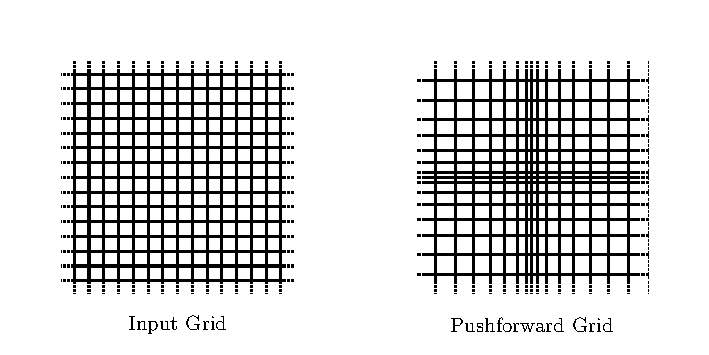
\includegraphics{figures/pushforward_grids/rectangular/rectangular.pdf}

}

\subcaption{\label{fig-pushforward-grids1}}

\end{minipage}%
%
\begin{minipage}{0.05\linewidth}
~\end{minipage}%
\newline
\begin{minipage}{0.05\linewidth}
~\end{minipage}%
%
\begin{minipage}{0.90\linewidth}

\centering{

\captionsetup{labelsep=none}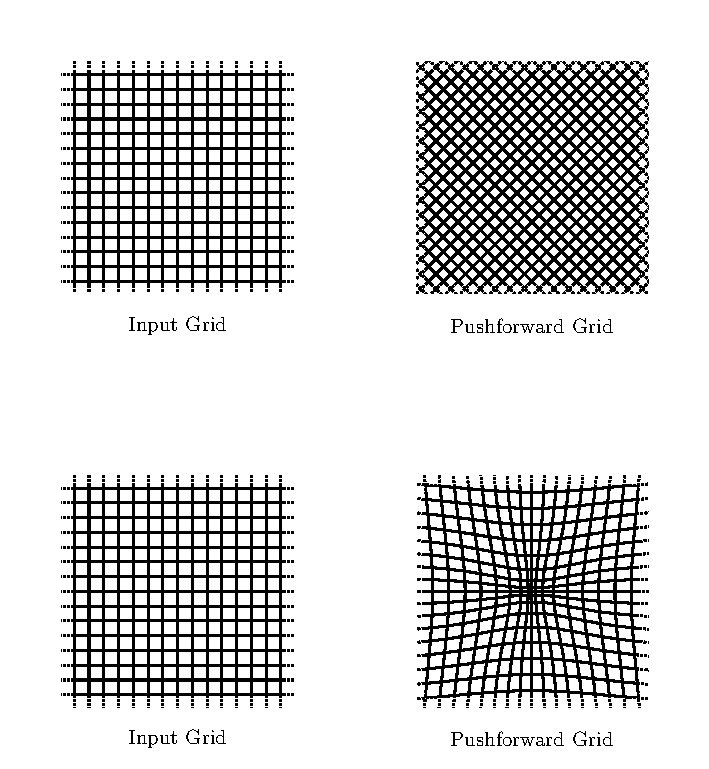
\includegraphics{figures/pushforward_grids/warped/warped.pdf}

}

\subcaption{\label{fig-pushforward-grids2}}

\end{minipage}%
%
\begin{minipage}{0.05\linewidth}
~\end{minipage}%

\caption{\label{fig-pushforward-grids}Maps between metric product spaces
may or may not preserve the individual components, and this has
consequences for how metric-informed grids transform. (a) Maps between
metric product spaces that do preserve the product structure transform
rectangular grids into rectangular grids. (b) On the other hand, maps
that mix the components transform rectangular grids into grids that
appear rotated, skewed, or otherwise warped.}

\end{figure}%

The behavior of component-preserving functions is completely determined
by the behavior of the component functions. For example, a
component-preserving function is injective, surjective, or bijective if
and only if all of the component functions are injective, surjective, or
bijective.

\subsection{Partial Evaluation}\label{partial-evaluation}

Fully evaluating a function on a product space requires specifying a
point in \emph{every} component space. For instance, in order to
evaluate the function \[
f: X_{1} \times X_{2} \rightarrow Y,
\] we need to specify both \(\tilde{x}_{1} \in X_{1}\) and
\(\tilde{x}_{2} \in X_{2}\), \[
f(\tilde{x}_{1}, \tilde{x}_{2}) = y \in Y.
\]

Providing only one component point leaves an empty slot in the input
product space that we need to fill in order to complete the evaluation.
For example, \(f(\tilde{x}_{1}, x_{2})\) is missing an a point in
\(X_{2}\) and \(f(x_{1}, \tilde{x}_{2})\) is missing a point in
\(X_{1}\). That empty slot, however, defines a relationship between the
missing inputs and the output space.

Specifically, \(f(\tilde{x}_{1}, x_{2})\) implicitly defines a function
that maps input points in the cross section
\(\{ \tilde{x}_{1} \} \times X_{2}\) to output points in \(Y\).
Similarly, \(f(x_{1}, \tilde{x}_{2})\) implicitly defines a function
that maps input points in the cross section
\(X_{1} \times \{ \tilde{x}_{2} \}\) to output points in \(Y\).

More generally, consider the subsequence of component indices \[
\mathsf{i}
=
( i_{1}, \ldots, i_{J} )
\] and corresponding component elements \[
\tilde{x}_{ \mathsf{i} } =
( \tilde{x}_{i_{1}}, \ldots, \tilde{x}_{i_{J}} ).
\] Inputting \(\tilde{x}_{ \mathsf{i} }\) into a function
\begin{alignat*}{6}
f :\; & X^{1:I} & &\rightarrow& \; & Y &
\\
& (x_{1}, \ldots, x_{i}, \ldots, x_{I}) & &\mapsto&
& y = f(x_{1}, \ldots, x_{i}, \ldots, x_{I}) &
\end{alignat*} defines a new function whose inputs are restricted to the
corresponding cross section, \begin{alignat*}{6}
f_{ \tilde{x}_{ \mathsf{i} } } :\; &
X^{ \mathsf{i}^{c} } \times \tilde{x}_{ \mathsf{i} } &
&\rightarrow& \; & Y &
\\
& (x_{1}, \ldots, x_{i_{1} - 1}, x_{i_{1} + 1}, \ldots, & &\mapsto&
& y = f(x_{1}, \ldots, x_{i_{1} - 1}, \tilde{x}_{i_{1}}, x_{i_{1} + 1}, \ldots, &
\\
& \;\, x_{i_{J} - 1}, x_{i_{J} + 1}, \ldots, x_{I} \quad\quad) & & &
& \quad\quad\quad x_{i_{J} - 1}, \tilde{x}_{i_{J}}, x_{i_{J} + 1}, \ldots, x_{I} \quad\quad) &.
\end{alignat*}

If we identify the cross sections with corresponding thinned product
space, \[
X^{ \mathsf{i}^{c} } \times \tilde{x}_{ \mathsf{i} }
\cong
X^{ \mathsf{i}^{c} },
\] then this procedure defines functions \[
f_{ \tilde{x}_{ \mathsf{i} } } :
X^{ \mathsf{i}^{c} } \rightarrow Y.
\]

This procedure is generally known as \textbf{partial evaluation},
although in computer science it is often referred to as
\textbf{Currying}. Besides the multi-index notation I use here, \[
f_{ \tilde{x}_{ \mathsf{i} } },
\] it is not uncommon to see notation like \[
f(\cdot \mid \tilde{x}_{i_{1}}, \ldots, \tilde{x}_{i_{J}}),
\] where \(\cdot\) represents a remaining, unbound input variable. One
might also encounter notation that explicitly writes out all of the
bound and unbound variables, \[
f(
  x_{1}, \ldots,
  x_{i_{1} - 1}, \tilde{x}_{i_{1}}, x_{i_{1} + 1}, \ldots,
  x_{i_{J} - 1}, \tilde{x}_{i_{J}}, x_{i_{J} + 1}, \ldots,
  x_{I}
).
\] While this latter notation is most direct, it quickly becomes
ungainly when working with more than a few components.

Partial evaluation of functions is often taken for granted in practical
applications. Explicitly acknowledging it, however, can help us better
understand less obvious constructions.

For instance, consider a space \(X\) equipped with a binary addition
operator \begin{alignat*}{6}
+ :\; & X \times X& &\rightarrow& \; & X &
\\
& x_{1}, x_{2} & &\mapsto& & x_{1} + x_{2} &.
\end{alignat*} Partially evaluating this function on the first input
component effectively defines a function \begin{alignat*}{6}
t_{\tilde{x}_{1}} :\; &X& &\rightarrow& \; & X &
\\
& x_{2} & &\mapsto& & \tilde{x}_{1} + x_{2} &.
\end{alignat*} This new function \emph{translates} each point in \(X\)
by \(\tilde{x}_{1}\). Unsurprisingly, \(t_{\tilde{x}_{1}}\) is referred
to as a translation operator.

Similarly, if we have a space \(X\) equipped with a binary
multiplication operator \begin{alignat*}{6}
\cdot :\; & X \times X& &\rightarrow& \; & X &
\\
& x_{1}, x_{2} & &\mapsto& & x_{1} \cdot x_{2} &,
\end{alignat*} then partial evaluation effectively defines a function
\begin{alignat*}{6}
s_{\tilde{x}_{1}} :\; &X& &\rightarrow& \; & X &
\\
& x_{2} & &\mapsto& & \tilde{x}_{1} \cdot x_{2} &.
\end{alignat*} This new function \emph{scales} each point in \(X\) by
\(\tilde{x}_{1}\). Fittingly, \(s_{\tilde{x}_{1}}\) is often referred to
as a scaling operator.

In many applications, translations and scalings appear to be intuitive.
Partial evaluation allows us to formalize that intuition, which can then
helps us recognize its limitations and consequences. For example,
translation isn't well-defined on a space that isn't equipped with the
right algebraic structure!

\section{Prototypical Product Spaces}\label{prototypical-product-spaces}

Most of the spaces that we encounter in practical applications are
product spaces built up from the prototypical spaces that we reviewed in
\href{http://www.symplectomorphic.com/assets/chapters_html/spaces.html\#sec:proto-spaces}{Chapter
2, Section 2}. In particular, these product spaces combine finite sets,
integers, and real lines together. That said, there are a few product
spaces worth particular note.

\subsection{Power Spaces}\label{power-spaces}

Often we are interested not in any single point of a space \(X\), but
rather multiple points at the same time. The selection of \(I\) distinct
points from the same space can be modeled by replicating the space \(I\)
times and then using those replications as components of a product
space, \[
X^{I} = X \times \ldots \times X = \prod_{i = 1}^{I} X.
\] This construction is often referred to as a \textbf{replicated
product space}, \textbf{identical product space}, or \textbf{power
space}.

We have already encountered this construction in a few places. For
example, we defined binary algebraic operator over the space \(X\) as
mapping two points in \(X\) into a single point in \(X\). That input
space of pairs of points was denoted \(X \times X\), which is just a
binary power space with a separate copy of \(X\) for each input.

Similarly, sequences of \(I\) points from a given space, \[
\{ x_{1}, \ldots, x_{i}, \ldots, x_{I} \},
\] can be defined as points of the power space \(X^{I}\). Allowing \(I\)
to approach countable infinity allows for arbitrarily long sequences.

One potential difficulty that can arise when working with power spaces
is distinguishing between the different copies of the base space \(X\)
that form the components. In particular, any notation that might
differentiate between the individual copies a single space, such as
ticks or integer indices, can also be confused as defining different
spaces entirely. Depending on the context, for instance,
\(X_{1} \times X_{2}\) might be used to denote both a product space
comprised of two \emph{different} component spaces or power space
comprised of two copies of the \emph{same} base space.

In practice, the most robust approach is typically to label each
component space with an integer index and then explicitly communicate
which, if any, component spaces are identical.

\subsection{Multivariate Real Numbers}\label{multivariate-real-numbers}

Combining \(I\) real lines together defines the \textbf{multivariate
real numbers}, \[
\mathbb{R}^{I} = \prod_{i = 1}^{I} \mathbb{R}.
\] This is also referred to as a \textbf{real space} or an
\textbf{\(I\)-dimensional Euclidean space}.

The multivariate real numbers inherit the identity crisis of the real
lines from which they are built. If we take the rigid real line
perspective, for instance, then there will be infinitely many
multivariate real numbers: different choices of component ordering,
algebraic, and metric structures define distinct product spaces.

On the other hand, if we assume the flexible real line perspective, then
then multivariate real numbers will correspond to a single, flexible
space. In this case, each distinct configuration of the component real
lines defines a different configuration of the corresponding product
space. Following the real line terminology, I will refer to these as
rigid real spaces and flexible real spaces, respectively.

To visually summarize the structure of a real space, we can extend
metric grids defined over the component spaces across the other
component spaces and then overlay them to form a rectangular \emph{mesh}
(Figure~\ref{fig-real_space_grid}).

\begin{figure}

\centering{

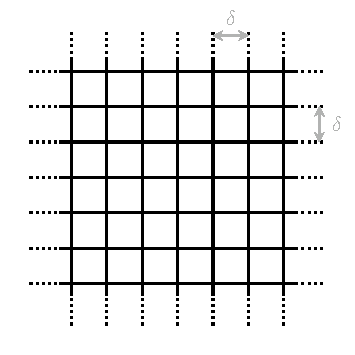
\includegraphics[width=0.5\textwidth,height=\textheight]{figures/real_space_grid/real_space_grid.pdf}

}

\caption{\label{fig-real_space_grid}Extending component grids into the
product space defines a rectangular mesh that visually communicate the
product metric structure. Here \(\mathbb{R}^{2}\) is represented by a
two-dimensional mesh.}

\end{figure}%

As we discussed in \hyperref[sec:rect-cyl]{Section 3.1}, the real space
\(\mathbb{R}^{2}\) is the one space where rectangular subsets actually
correspond to Euclidean rectangles.

\section{Conclusion}\label{conclusion}

The construction of product spaces defines a systematic way to work with
multiple spaces at the same time. Because product spaces define the
sophisticated spaces we need for many practical applications, we will
need to be comfortable with their structure and manipulation.

Working with more than a few component spaces does require some careful
organization. In some cases, we can explicitly enumerate each component
set with distinct variable names. In others, we can fall back on more
flexible tools like multi-index notation.

\section*{Acknowledgements}\label{acknowledgements}
\addcontentsline{toc}{section}{Acknowledgements}

I thank Alexander Noll, Pietro Monticone, and and Léo Burgund for
helpful comments.

A very special thanks to everyone supporting me on Patreon: Adam
Fleischhacker, Adriano Yoshino, Alan Chang, Alessandro Varacca,
Alexander Bartik, Alexander Noll, Alexander Petrov, Alexander Rosteck,
Anders Valind, Andrea Serafino, Andrew Mascioli, Andrew Rouillard,
Andrew Vigotsky, Angie\_Hyunji Moon, Ara Winter, Austin Rochford, Austin
Rochford, Avraham Adler, Ben Matthews, Ben Swallow, Benjamin Glemain,
Bradley Kolb, Brynjolfur Gauti Jónsson, Cameron Smith, Canaan Breiss,
Cat Shark, Charles Naylor, Chase Dwelle, Chris Zawora, Christopher
Mehrvarzi, Chuck Carlson, Colin Carroll, Colin McAuliffe, Cruz, Damien
Mannion, Damon Bayer, dan mackinlay, Dan Muck, Dan W Joyce, Dan Waxman,
Dan Weitzenfeld, Daniel Edward Marthaler, Daniel Rowe, Darshan Pandit,
Darthmaluus , David Burdelski, David Galley, David Humeau, David Wurtz,
dilsher singh dhillon, Doug Rivers, Dr.~Jobo, Dr.~Omri Har Shemesh, Ed
Cashin, Ed Henry, Edgar Merkle, edith darin, Eric LaMotte, Erik Banek,
Ero Carrera, Eugene O'Friel, Felipe González, Fergus Chadwick, Finn
Lindgren, Florian Wellmann, Francesco Corona, Geoff Rollins, Greg
Sutcliffe, Guido Biele, Hamed Bastan-Hagh, Haonan Zhu, Hector Munoz,
Henri Wallen, hs, Hugo Botha, Håkan Johansson, Ian Costley, Ian Koller,
idontgetoutmuch, Ignacio Vera, Ilaria Prosdocimi, Isaac Vock, J, J
Michael Burgess, Jair Andrade, James Hodgson, James McInerney, James
Wade, Janek Berger, Jason Martin, Jason Pekos, Jason Wong, Jeff Burnett,
Jeff Dotson, Jeff Helzner, Jeffrey Erlich, Jesse Wolfhagen, Jessica
Graves, Joe Wagner, John Flournoy, Jonathan H. Morgan, Jonathon Vallejo,
Joran Jongerling, Joseph Despres, Josh Weinstock, Joshua Duncan, Joshua
Griffith, Josué Mendoza, JU, Justin Bois, Karim Naguib, Karim Osman,
Kejia Shi, Kevin Foley, Kristian Gårdhus Wichmann, Kádár András, lizzie
, LOU ODETTE, Marc Dotson, Marcel Lüthi, Marek Kwiatkowski, Mark
Donoghoe, Mark Worrall, Markus P., Martin Modrák, Matt Moores, Matthew,
Matthew Kay, Matthieu LEROY, Maurits van der Meer, Merlin Noel
Heidemanns, Michael DeWitt, Michael Dillon, Michael Lerner, Mick Cooney,
Márton Vaitkus, N Sanders, Name, Nathaniel Burbank, Nic Fishman,
Nicholas Clark, Nicholas Cowie, Nick S, Nicolas Frisby, Octavio Medina,
Ole Rogeberg, Oliver Crook, Olivier Ma, Pablo León Villagrá, Patrick
Kelley, Patrick Boehnke, Pau Pereira Batlle, Peter Smits, Pieter van den
Berg , ptr, Putra Manggala, Ramiro Barrantes Reynolds, Ravin Kumar, Raúl
Peralta Lozada, Riccardo Fusaroli, Richard Nerland, RLW, Robert Frost,
Robert Goldman, Robert kohn, Robert Mitchell V, Robin Taylor, Ross
McCullough, Ryan Grossman, Rémi , S Hong, Scott Block, Scott Brown, Sean
Pinkney, Sean Wilson, Seth Axen, shira, Simon Duane, Simon Lilburn,
Srivatsa Srinath, sssz, Stan\_user, Stefan, Stephanie Fitzgerald,
Stephen Lienhard, Steve Bertolani, Stone Chen, Susan Holmes, Svilup,
Sören Berg, Tao Ye, Tate Tunstall, Tatsuo Okubo, Teresa Ortiz, Thomas
Lees, Thomas Vladeck, Tiago Cabaço, Tim Radtke, Tobychev , Tom McEwen,
Tony Wuersch, Utku Turk, Virginia Fisher, Vitaly Druker, Vladimir
Markov, Wil Yegelwel, Will Farr, Will Tudor-Evans, woejozney, Xianda
Sun, yolhaj , yureq , Zach A, Zad Rafi, and Zhengchen Cai.

\section*{License}\label{license}
\addcontentsline{toc}{section}{License}

The text and figures in this chapter are copyrighted by Michael
Betancourt and licensed under the CC BY-NC 4.0 license:

https://creativecommons.org/licenses/by-nc/4.0/



\end{document}
